\section{Output Data Comparison}
Data presented in section~\ref{sec:Results} were compared with data obtained from an identical situation simulated in DIALux software, where a street project has been created using luminaires Atos A1. The street project output illuminances were calculated by DIALux according to~\cite{CSN_EN_13201-3} as seen in figure~\ref{fig:lumIntDistr} and the output in lux can be found in table~\ref{tab:DialuxOneSideLamps}.

\begin{figure}[htb]
  \centering
  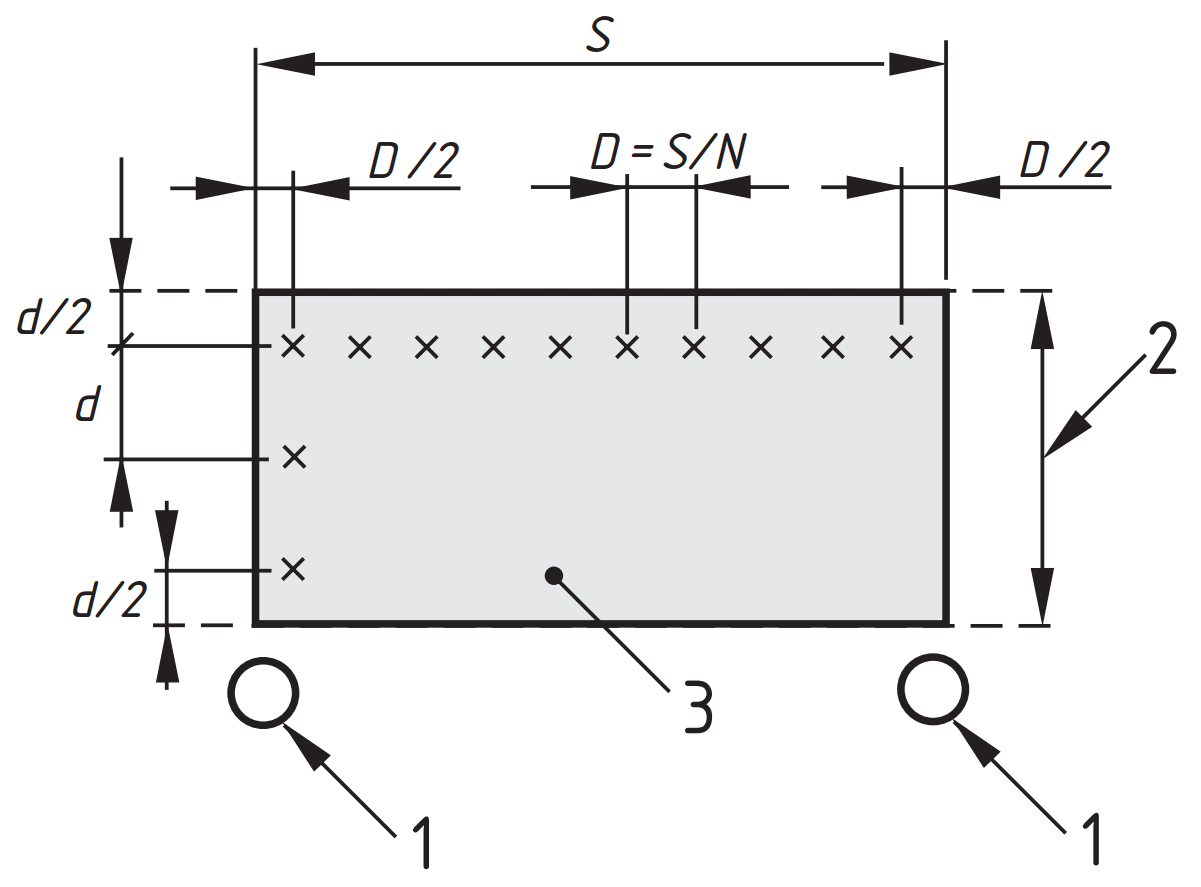
\includegraphics[width=0.8\columnwidth]{13201-3_points}
  \caption{Calculation points on relevant area \cite{CSN_EN_13201-3}}
  \label{fig:lumIntDistr}
	\begin{description}
		\item[1] luminaire
		\item[2] width of relevant area $W_{r}$
		\item[3] field of calculation
		\item[x] denotes lines of calculation points in the transverse and longitudinal directions
	\end{description}
\end{figure}

\begin{table}[htb]
	\renewcommand{\arraystretch}{1.3}
	\caption{DIALux calculated illuminances in lux for one side lamp placement at the surface of the road}
 	\label{tab:DialuxOneSideLamps}
	\centering
  \begin{tabular}{ l || c | c | c | c | c | c | c | c | c | c }
    \hline
    \textbf{(m)} & 1.3 & 3.9 & 6.5 & 9.1 & 11.7 & 14.3 & 16.9 & 19.5 & 22.1 & 24.7\\ \hline \hline
    2.5 & 11 & 9.56 & 7.09 & 5.57 & 4.48 & 4.48 & 5.57 & 7.09 & 9.56 & 11\\ \hline
		1.5 & 12 & 10 & 7.08 & 5.36 & 4.14 & 4.14 & 5.36 & 7.08 & 10 & 12\\ \hline
		0.5 & 13 & 10 & 7.01 & 5.10 & 3.85 & 3.85 & 5.10 & 7.01 & 10 & 13\\ \hline
  \end{tabular}
\end{table}